\documentclass[]{homework}
\usepackage{tikz}
\usepackage{wrapfig}

\begin{document}


\homework{3}{Feb. 11, 2021}


\begin{problem}{1}

  Consider the ellipse given by

  \vspace{-1em}
  \begin{minipage}[t]{\linewidth}
  \begin{wrapfigure}{r}{4.5cm}
    \vspace{-2.5em}
    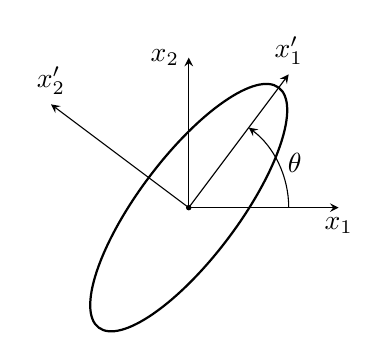
\begin{tikzpicture}[>=stealth]
      \fill (0,0) circle (1pt);
      \draw [thick,rotate=53.13] (0,0) ellipse (0.75in and 0.25in);
      \draw [->] (0,0) -- (0.75in,0) node [below] {$x_1$};
      \draw [->] (0,0) -- (0,0.75in) node [left] {$x_2$};
      \draw [->,rotate=53.13] (0,0) -- (0.75in,0) -- ++ (6pt,0) node [above]
            {$x_1'$};
      \draw [->,rotate=53.13+90] (0,0) -- (0.75in,0) -- ++ (8pt,0) node
            [above] {$x_2'$};
      \draw [->] (0.5in,0) arc (0:53.13:0.5in);
      \path (53.13/2:0.5in) node [right] {$\theta$};
    \end{tikzpicture}
  \end{wrapfigure}

  \begin{equation}
    14 x_1^2 - 4 x_1 x_2 + 11 x_2^2 = 25.\nonumber
  \end{equation}


  This ellipse is shown at the right.  We want to find the principle axes
  of this ellipse represented by $x_1'$ and $x_2'$ in the figure.  In this
  problem \textbf{all calculations should be done by hand} unless
  otherwise noted. If your linear algebra is rusty, feel free to use 
  any resources you like as a reference.
  \end{minipage}

  \begin{subproblem}{a}
    We can write the equation for the ellipse as a matrix equation of
    the form
    \[ \transpose{\vec x} \mat A \vec x
    =
    \begin{pmatrix} x_1 & x_2 \end{pmatrix}
    \begin{pmatrix} a_{00} & a_{01} \\ a_{01} & a_{11} \end{pmatrix}
    \begin{pmatrix} x_1 \\ x_2 \end{pmatrix}
    = 25.
    \]
    Notice that I have written $\mat A$ as a \emph{symmetric} matrix.
    Write down the matrix $\mat A$.
  \end{subproblem}
  \begin{subproblem}{b}
    Calculate the eigenvalues, $\lambda_n$, of $\mat A$.  Clearly show how
    you calculate the eigenvalues. \note{ Despite how it may appear, the
      coefficients of the ellipse have been chosen to lead to simple
      eigenvalues.}
  \end{subproblem}
  \begin{subproblem}{c}
    Calculate the eigenvectors, $\vec v_n$, of $\mat A$.  Remember that
    eigenvectors are normalized so that $|\vec v_n|=1$. \note{ Again, the
      coefficients have been chosen so that the eigenvectors will have
      ``simple'' values.}
  \end{subproblem}
  \begin{subproblem}{d}
    Consider another matrix $\mat B$, which contains the eigenvectors of $\mat A$
    as its columns.
    Show that $\mat B$ diagonalizes the matrix $\mat A$.  To do this,
    calculate the product $\mat D = \transpose{\mat B}\mat A\mat B$.
    \note{ What diagonal matrix should this product produce?
    Make sure your answer agrees with this.}
  \end{subproblem}
  \begin{subproblem}{e}
    Since $\mat A$ is symmetric, this matrix $\mat B$ should be orthogonal.
    This means $\inverse{\mat B} = \transpose{\mat B}$.  To show this
    calculate the product $\transpose{\mat B}\mat B$. \note{ What should
      the answer be?  Make sure your answer agrees with this.}
  \end{subproblem}
  \begin{subproblem}{f}
    The matrix $\mat B$ is a rotation matrix that transforms between the
    two coordinate systems shown in the figure.  Explicitly, $\vec x' =
    \transpose{\mat B} \vec x$.  Determine the angle, $\theta$, between the
    original $x_1$-axis and the new $x_1'$-axis.
  \end{subproblem}
  \begin{subproblem}{g}
    Finally, write the ellipse in standard form in terms of the principle
    axes
    \[ \left( \frac{x_1'}{\alpha_1} \right)^2 + \left( \frac{x_2'}{\alpha_2}
    \right)^2 = 1 .\]
    In other words, determine $\alpha_1$ and $\alpha_2$.
  \end{subproblem}


\end{problem}



\begin{problem}{2}
  Even when a matrix is not singular, it can still be difficult to work with
  numerically.  The condition number of a matrix, $\mat A$, is denoted by
  $\kappa(\mat A)$.  If $\kappa$ is large we call the matrix \emph{ill
    conditioned}.  Roughly, if the condition number is of the form
  $\kappa(\mat A)\sim 10^k$ then we expect to lose up to $k$ digits of
  accuracy in addition to the normal loss of accuracy in an algorithm
  involving $\mat A$.  We will calculate the condition number
  as\footnote{This is not the most general definition but is sufficient for our
    purposes.}
  \[ \kappa(\mat A) = \frac{\max\left( |\lambda(\mat A)|
    \right)}{\min\left( |\lambda(\mat A)| \right)}, \]
  where $\lambda(\mat A)$ are the eigenvalues of $\mat A$.  The Hilbert
  matrix is an example of a non-singular but ill conditioned matrix.  It
  has elements $A_{ij} = 1/(i+j+1)$ so that $A_{00}=1$, $A_{01}=1/2$,
  \textit{etc}.  In python we may easily construct this matrix by hand but
  we do not need to!  We can instead use
  \code{scipy.linalg.hilbert()}. \note{ A number of other, standard
    matrices are defined too.}
  \begin{subproblem}{a}
    Calculate the condition number $\kappa(A)$ for the $10\times10$ Hilbert
    matrix.  Since $\mat A$ is symmetric you should use
    \code{scipy.linalg.eigh} for this purpose.
  \end{subproblem}
  \begin{subproblem}{b}
    Calculate the inverse of $\mat A$ using \code{scipt.linalg.inv}
    and determine the maximum absolute
    error in $\inverse{\mat A}\mat A-\mat I$.
  \end{subproblem}
  \begin{subproblem}{c}
    An alternative way to calculate the inverse is to use the matrix of
    eigenvectors, $\mat B$.  Since $\mat A$ is symmetric we know that
    $\transpose{\mat B}\mat A\mat B = \mat D$ is the diagonal matrix of the
    eigvenvalues.  With this we may calculate the inverse as
    \[ \inverse{\mat A} = \mat B\inverse{\mat D}\transpose{\mat B}. \]
    Using this expression repeat the previous part.  We should find in
    these two parts that the maximum error is huge compared to the expected
    numerical error.
    \hint{Calculating the inverse of a diagonal matrix is very easy to do
      by hand.}
  \end{subproblem}
\end{problem}


\begin{problem}{3}
  Complete the Jupyter notebook assignment.
\end{problem}


\end{document}

